\section{Seifert}

\tikzset{
  plusnode/.style={circle, draw=green!60, fill=yellow!5, very thick, minimum size=5mm, scale=0.8, font=\color{green!80!red}\bfseries},
  minusnode/.style={circle, draw=blue!60, fill=orange!5, very thick, minimum size=5mm, scale=0.8, font=\color{blue!80!red}\bfseries}
}

Na \cref{pow61} jest powierzchnia Seiferta $6_1$, kolory oznaczają pętelki-generatory.

Moduł Alexandera wychodzi $\Z[\Z]/(-2t^2+5t-2)$, czyli nic niezwykłego.

\begin{figure}[h]\centering
  \begin{tikzpicture}
  \draw (0,0) circle (1);
  \draw (0,0) ellipse (2.5 and 3.5);
  \draw (6, 0) circle (1);
  \draw (4.5, 3) circle (1);
  \draw (4.5, -3) circle (1);
  
  \coordinate (firstEnd) at ({2.5 * cos(8)}, {3.5 * sin(8)});
  \coordinate (secondEnd) at ({2.5 * cos(-8)}, {3.5 * sin(-8)});

  \draw ({cos(30)}, {sin(30)}) to [out=0, in=180] (secondEnd);
  \fill[white] (1.7, 0) circle (4pt);
  \draw ({cos(-30)}, {sin(-30)}) to[out=0, in=180] (firstEnd);
  \draw[ultra thick, white] ({cos(29)}, {sin(29)}) arc (29:-29:1);

  \coordinate (firstEnd) at ({-2.5 * cos(8)}, {3.5 * sin(8)});
  \coordinate (secondEnd) at ({-2.5 * cos(-8)}, {3.5 * sin(-8)});

  \draw ({-cos(-30)}, {sin(-30)}) to[out=180, in=0] (firstEnd);
  \fill[white] (-1.7, 0) circle (4pt);
  \draw ({-cos(30)}, {sin(30)}) to[out=180, in=0] (secondEnd);
  \draw[ultra thick, white] ({-cos(29)}, {sin(29)}) arc (180-29:180+29:1);

  \coordinate (a1) at ({2.5 * cos(45)}, {3.5 * sin(45)});
  \coordinate (a2) at ({2.5 * cos(70)}, {3.5 * sin(70)});
  
  \draw[ultra thick, white] (a1) arc (45:70:2.5 and 3.5);

  \begin{scope}[shift={(4.5, 3)}] 
    \coordinate (a3) at ({-cos(30)}, {sin(30)});
    \coordinate (a4) at ({-cos(-30)}, {sin(-30)});
    \draw[ultra thick, white] (a3) arc (180-30:180+30:1);
  \end{scope}
  
  \begin{scope}[shift={(4.5, -3)}] 
    \coordinate (a5) at ({-cos(30)}, {sin(30)});
    \coordinate (a6) at ({-cos(-30)}, {sin(-30)});
    \draw[ultra thick, white] (a5) arc (180-30:180+30:1);
  \end{scope}
  
  \coordinate (a7) at ({2.5 * cos(-45)}, {3.5 * sin(-45)});
  \coordinate (a8) at ({2.5 * cos(-70)}, {3.5 * sin(-70)});

  \draw[ultra thick, white] (a7) arc (-45:-70:2.5 and 3.5);

  %\foreach \i in {1,...,8} \fill (a\i) circle (4pt) node [above] {\i};

  \draw[name path=a1-3] (a1) to[out=70, in=180] (a3);
  \draw[white, name path=a2-4] (a2) to[out=45, in=180] (a4);
  \path [name intersections={of=a1-3 and a2-4, by=A1}];
  \fill[white] (A1) circle (4pt);
  \draw (a2) to[out=45, in=180] (a4);
  
  \draw[white, name path=a7-6] (a7) to[out=-45, in=180] (a6);
  \draw[name path=a8-5] (a8) to[out=-70, in=180] (a5);
  \path [name intersections={of=a7-6 and a8-5, by=A2}];
  \fill[white] (A2) circle (4pt);
  \draw (a7) to[out=-45, in=180] (a6);

  \begin{scope}[shift={(6, 0)}]
    \coordinate (b1) at ({cos(90-30)}, {sin(90-30)});
    \coordinate (b2) at ({cos(90+30)}, {sin(90+30)});

    \coordinate (b3) at({cos(-90-30)}, {sin(-90-30)});
    \coordinate (b4) at({cos(-90+30)}, {sin(-90+30)});
  \end{scope}

  \begin{scope}[shift={(4.5, 3)}]
    \coordinate (b5) at ({cos(-90+30)}, {sin(-90+30)});
    \coordinate (b6) at (1, 0);
  \end{scope}

  \begin{scope}[shift={(4.5, -3)}]
    \coordinate (b7) at (1, 0);
    \coordinate (b8) at ({cos(90-30)}, {sin(90-30)});
  \end{scope}
  
  %\foreach \i in {1,...,8} \fill (b\i) circle (4pt) node [above] {\i};
  
  \draw[white, ultra thick] (b6) arc (0:-60:1);
  \draw[white, ultra thick] (b2) arc (120:60:1);
  \draw[ultra thick, white] (b3) arc (-90-30:-90+30:1);
  \draw[ultra thick, white] (b8) arc (60:0:1);

  \draw[name path=b5-1] (b5) to[out=-60, in=90] (b1);
  \draw[name path=b6-2, white] (b6) to[out=0, in=90] (b2);
  \path[name intersections={of=b5-1 and b6-2, by=B1}];
  \fill[white] (B1) circle (4pt);
  \draw (b6) to[out=0, in=90] (b2);

  \draw[name path=b7-3] (b7) to[out=60, in=-90] (b3);
  \draw[name path=b8-4, white] (b8) to[out=0, in=-90] (b4);
  \path[name intersections={of=b7-3 and b8-4, by=B2}];
  \fill[white] (B2) circle (4pt);
  \draw (b8) to[out=0, in=-90] (b4);

  \draw[thick, purple, ->] (4.5, 3) to[out=180, in=0] 
    (A1) to[out=180, in=90] 
    (1.5, 2);
  \draw[thick, purple, ->] (1.5, 2) to[out=-90, in=90]
    (1.5, -2);
  \draw[thick, purple, ->] (1.5, -2) to[out=-90, in=180]
    (A2) to[out=0, in=180]
    (4.5, -3);
  \draw[thick, purple, ->] (4.5, -3) to[out=0, in=240]
    (B2) to[out=60, in=-90] 
    (6, 0);
  \draw[purple, thick, ->] (6, 0) to[out=90, in=-60]
    (B1) to[out=120, in=0]
    (4.5, 3);

  \draw[thick, purple, ->] (0,-0.3) to[out=160, in=-70] (-2.5, 0.6);
  \draw[thick, purple, ->] (-2.5, 0.6) to[out=90, in=180] (0, 1.5);
  \draw[thick, purple, ->] (0, 1.5) to[out=0, in=90] (2.5, 0.6);
  \draw[thick, purple, ->] (2.5, 0.6) to[out=-110, in=20] (0,-0.3);

  \node at (0, -0.7) {$\color{purple}a$};
  \node at (6.4, 0) {$\color{purple}b$};

  \node[plusnode] at (0,0.4) {$+$};
  \node[plusnode] at (5.45, 0) {$+$};
  \node[plusnode] at (-1, 2.3) {$+$};

  \node[minusnode] at (4.2, 3.5) {$-$};
  \node[minusnode] at (4.2, -3.5) {$-$};
\end{tikzpicture}

\caption{\label{pow61}Powierzchnia Seiferta $6_1$.}
\end{figure}


Powierzchnia Seiferta węzła $9_{46}$ jest z kolei na \cref{pow946} i nie wychodzi ładnie. To znaczy, relacje po rozpisaniu wyglądają następująco (nad znakami równości z których czerwonych pętelek przychodzą, pozostałe to obserwacje obrazku):
\begin{align*}
  ta^- &\overset{a}{=} X-f^--a^-\\ 
  0&\overset{b}{=}-Y+E+a^-\\ 
  tX+tC&\overset{c}{=}c^+\\ 
  -tY&\overset{d}{=}c^+ \\ 
  tZ-tE&\overset{e}{=}-Y+G\\ 
  tf^- &\overset{f}{=}Z-c^++X\\ 
  C-G&=c^+\\ 
  0&=X+Y+Z
\end{align*}
\begin{figure}[h]\centering
  \begin{tikzpicture}
  \begin{scope}
    \draw (0,0) circle (1);
    \draw (0,0) ellipse (2.5 and 3.5);
    
    \coordinate (B1) at ({cos(180-20)-1.5}, {sin(180-20)});
    \coordinate (A1) at ({cos(180+20)-1.5}, {sin(180+20)});

    \coordinate (B0) at (360/3-90:2.5 and 3.5);
    \coordinate (A0) at (360/3+20-90:2.5 and 3.5);

    \coordinate (B2) at (2*360/3-30+100:2.5 and 3.5);
    \coordinate (A2) at (2*360/3-10+100:2.5 and 3.5);

    \foreach \i in {0,1,2} {
      \coordinate (a\i) at (\i*360/3 + 60+20:1);
      \coordinate (b\i) at (\i*360/3 + 60-20:1);

      % \fill (a\i) circle (4pt) node [above] {a\i};
      % \fill (b\i) circle (4pt) node [above] {b\i};
      %
      % \fill (A\i) circle (4pt) node [above] {A\i};
      % \fill (B\i) circle (4pt) node [above] {B\i};
    }

    \coordinate (c1) at (90+20:2.5 and 3.5);
    \coordinate (c2) at (90-20:2.5 and 3.5);
    \coordinate (c3) at (15:2.5 and 3.5);
    \coordinate (c4) at (-15:2.5 and 3.5);
    \coordinate (c5) at (-90+20:2.5 and 3.5);
    \coordinate (c6) at (-90-20:2.5 and 3.5);

    % \foreach \i in {1,..., 6} \fill (c\i) circle (4pt) node[above] {c\i};
    \draw[ultra thick,white] (c1) arc (110:70:2.5 and 3.5);
    \draw[ultra thick,white] (c3) arc (15:-15:2.5 and 3.5);
    \draw[ultra thick,white] (c5) arc (-70:-110:2.5 and 3.5);
  \end{scope}

  
  \begin{scope}[shift={(7, 0)}]
    \draw (0,0) circle (1);
    \draw (0,0) ellipse (2.5 and 3.5);

    \coordinate (D0) at ({cos(-20)+1.5}, {sin(-20)});
    \coordinate (E0) at ({cos(20)+1.5}, {sin(20)});
    \coordinate (D1) at (360/3+10:2.5 and 3.5);
    \coordinate (E1) at (360/3+30:2.5 and 3.5);
    \coordinate (D2) at (2*360/3-30:2.5 and 3.5);
    \coordinate (E2) at (2*360/3-10:2.5 and 3.5);

    \foreach \i in {0,1,2} {
      \coordinate (d\i) at (\i*360/3-20:1);
      \coordinate (e\i) at (\i*360/3+20:1);

      % \fill (d\i) circle (4pt) node [above] {d\i};
      % \fill (e\i) circle (4pt) node [above] {e\i};
      %
      % \fill (D\i) circle (4pt) node [above] {D\i};
      % \fill (E\i) circle (4pt) node [above] {E\i};
    }

    \coordinate (f1) at (90-20:2.5 and 3.5);
    \coordinate (f2) at (90+20:2.5 and 3.5);
    \coordinate (f3) at (180-15:2.5 and 3.5);
    \coordinate (f4) at (180+15:2.5 and 3.5);
    \coordinate (f5) at (-90-20:2.5 and 3.5);
    \coordinate (f6) at (-90+20:2.5 and 3.5);
    
    \draw[ultra thick,white] (f2) arc (110:70:2.5 and 3.5);
    \draw[ultra thick,white] (f3) arc (180-15:180+15:2.5 and 3.5);
    \draw[ultra thick,white] (f6) arc (-70:-110:2.5 and 3.5);

    % \foreach \i in {1,..., 6} \fill (f\i) circle (4pt) node[above] {f\i};
  \end{scope}

  \draw[name path=c1-f2, white] (c1) to[out=90, in=90] (f2);
  \draw[name path=c2-f1] (c2) to[out=90, in=90] (f1);
  \path[name intersections={of=c1-f2 and c2-f1, by=CF1}];
  \fill[white] (CF1) circle (15pt);
  \draw (c1) to[out=90, in=90] (f2);

  \draw[name path=c5-f6] (c5) to[out=-90, in=-90] (f6);
  \draw[name path=c6-f5, white] (c6) to[out=-90, in=-90] (f5);
  \path[name intersections={of=c5-f6 and c6-f5, by=CF2}];
  \fill[white] (CF2) circle (15pt);
  \draw (c6) to[out=-90, in=-90] (f5);

  \draw[name path=c3-f4, white] (c3) to[out=0, in=180] (f4);
  \draw[name path=c4-f3] (c4) to[out=0, in=180] (f3);
  \path[name intersections={of=c3-f4 and c4-f3, by=CF3}];
  \fill[white] (CF3) circle (6pt);
  \draw (c3) to[out=0, in=180] (f4);

  \foreach \i in {0,2} {
    \draw[ultra thick, white] (e\i) arc (\i*120+20:\i*120-30:1);

    \draw[name path=u\i, white] (e\i) to[out=360/3*\i, in=180+\i*360/3] (D\i);
    \draw[name path=t\i] (d\i) to[out=360/3*\i, in=180+\i*360/3] (E\i);
    \path[name intersections={of={u\i} and {t\i}, by=DE\i}];
    \fill[white] (DE\i) circle (6pt);
    \draw (e\i) to[out=360/3*\i, in=180+\i*360/3] (D\i);
  }
  \foreach \i in {1} {
    \draw[ultra thick, white] (e\i) arc (\i*120+20:\i*120-30:1);

    \draw[name path=u\i] (e\i) to[out=360/3*\i, in=180+\i*360/3] (D\i);
    \draw[name path=t\i, white] (d\i) to[out=360/3*\i, in=180+\i*360/3] (E\i);
    \path[name intersections={of={u\i} and {t\i}, by=DE\i}];
    \fill[white] (DE\i) circle (6pt);
    \draw (d\i) to[out=360/3*\i, in=180+\i*360/3] (E\i);
  }


  \foreach \i in {1,2} {
    \draw[ultra thick, white] (a\i) arc (\i*120+60+20:\i*120+60+20-30:1);

    \draw[name path=s\i, white] (a\i) to[out=360/3*\i+60, in=\i*360/3-120] (B\i);
    \draw[name path=r\i] (b\i) to[out=360/3*\i+60, in=\i*360/3-120] (A\i);
    \path[name intersections={of={s\i} and {r\i}, by=AB\i}];
    \fill[white] (AB\i) circle (6pt);
    \draw (a\i) to[out=360/3*\i+60, in=\i*360/3-120] (B\i);
  }
  \foreach \i in {0} {
    \draw[ultra thick, white] (a\i) arc (\i*120+60+20:\i*120+60+20-30:1);

    \draw[name path=s\i] (a\i) to[out=360/3*\i+60, in=\i*360/3-120] (B\i);
    \draw[name path=r\i,white] (b\i) to[out=360/3*\i+60, in=\i*360/3-120] (A\i);
    \path[name intersections={of={s\i} and {r\i}, by=AB\i}];
    \fill[white] (AB\i) circle (6pt);
    \draw (b\i) to[out=360/3*\i+60, in=\i*360/3-120] (A\i);
  }

  \draw[thick, purple, ->] (CF1) to[out=180, in=90] (0, 3.5);
  \draw[thick, purple, ->] (0, 3.5) to[out=-90, in=160] (2.7, 0.5);
  \draw[thick, purple, ->] (2.7, 0.5) to[out=-20, in=180] (3.5, 0.05) to[out=0, in=200] (4.3, 0.5);
  \draw[thick, purple, ->] (4.3, 0.5) to[out=20, in=-90] (7, 3.5);
  \draw[thick, purple, ->] (7, 3.5) to[out=90, in=0] (CF1);
  \node at (3.7, 5) {$\color{purple}e$};
  
  \draw[thick, purple, ->] (CF2) to[out=180, in=-90] (0, -3.5);
  \draw[thick, purple, ->] (0, -3.5) to[out=90, in=200] (2.7, -0.5);
  \draw[thick, purple, ->] (2.7, -0.5) to[out=20, in=180] (3.5, -0.05) to[out=0, in=160] (4.3, -0.5);
  \draw[thick, purple, ->] (4.3, -0.5) to[out=-20, in=90] (7, -3.5);
  \draw[thick, purple, ->] (7, -3.5) to[out=-90, in=0] (CF2);
  \node at (3.7, -5) {$\color{purple}f$}; 



  \draw[thick, purple, ->] (0,0.5) to[out=210, in=0] ([yshift=2pt]AB1) 
  to[out=180, in=-90] (175:2.5 and 3.5)
  to[out=90, in=210] (-0.8, 1.8);
  \draw[thick, purple, ->] (-0.8, 1.8) to[out=30, in=90] (40:2.5 and 3.5) 
  to[out=-90, in=60] ([yshift=2pt]AB0) to[out=240, in=30] (0, 0.5);
  
  \draw[thick, purple, ->] (0, -0.5) to[out=150, in=0] ([yshift=-2pt]AB1) 
  to[out=180, in=90] (185:2.5 and 3.5)
  to[out=-90, in=150] (-0.8, -1.8);
  \draw[thick, purple, ->] (-0.8, -1.8) to[out=-30, in=-90] (-40:2.5 and 3.5)
  to[out=90, in=-60] ([yshift=-2pt]AB2) to[out=120, in=-30] (0, -0.5);


  \begin{scope}[shift={(7, 0)}]
    \draw[thick, purple, ->] (0,0.5) to[out=150, in=-60] ([yshift=2pt]DE1) 
    to[out=120, in=-90] (180-40:2.5 and 3.5)
    to[out=90, in=150] (0.8, 1.8);
    \draw[thick, purple, ->] (0.8, 1.8) to[out=-30, in=90] (5:2.5 and 3.5) 
    to[out=-90, in=-30] ([yshift=2pt]DE0) to[out=150, in=-30] (0, 0.5);
  
    \draw[thick, purple, ->] (0, -0.5) to[out=210, in=60] ([yshift=-2pt]DE2) 
    to[out=240, in=90] (180+40:2.5 and 3.5)
    to[out=-90, in=210] (0.8, -1.8);
    \draw[thick, purple, ->] (0.8, -1.8) to[out=30, in=-90] (-5:2.5 and 3.5)
    to[out=90, in=-30] ([yshift=-2pt]DE0) to[out=150, in=30] (0, -0.5);
  \end{scope}

  \node at (-0.8, 2.2) {$\color{purple}b$};
  \node at (-0.8, -2.2) {$\color{purple}a$};
  \node at (7.8, 2.2) {$\color{purple}d$};
  \node at (7.8, -2.2) {$\color{purple}c$};

  \draw[->, thick, blue] (2, 5.5) arc (170:-130:0.5 and 1);
  \node at (1.8, 6) {$\color{blue}Y$};

  \draw[->, thick, blue] (3, 0.9) arc (120:-120:0.5 and 1.1);
  \node at (3.1, 1.3) {$\color{blue}Z$};

  \draw[->, thick, blue] (2, -4.7) arc (170:-130:0.5 and 1);
  \node at (1.8, -5.2) {$\color{blue}X$};

  \draw[->, thick, blue] ([xshift=-6pt, yshift=6pt]AB0) arc (170:-110:0.3 and 0.7); 
  \node at ([yshift=-25pt, xshift=10pt]AB0) {$\color{blue}E$};

  \draw[->, thick, blue] ([yshift=10pt]DE1) arc (120:-180:0.3 and 0.7);
  \node at ([yshift=-25pt, xshift=-15pt]DE1) {$\color{blue}G$};

  \draw[->, thick, blue] ([yshift=10pt]DE0) arc (160:-150:0.3 and 0.7);
  \node at ([yshift=-25pt]DE0) {$\color{blue}C$};

  \node[plusnode] at (7,0) {$+$};
  \node[plusnode] at (8, 2.7) {$+$};
  \node[minusnode] at (0, 0) {$-$};
  \node[minusnode] at (-1, 2.7) {$-$};
\end{tikzpicture}

  \caption{\label{pow946}Powierzchnia Seiferta $9_{46}$.}
\end{figure}

Z tych równań wyciągam tylko tyle, że 
$$Z(1-t)+X(1-2t)+a^-(t^2+t)=0$$
oraz
$$Y(3t^2+2t-3)=X(1+t-t^2).$$
Moim zdaniem powinno wyjść coś z dwoma generatorami, ale jeszcze nie wymyśliłam jak je wyciągnąć.

\section{Relacja na macierzach}

% Nie wzięłam ze sobą zeszytu, w którym mazałam we Wrocławiu, więc musiałam ten problem od zera rozpisywać i coś mi się przestało zgadzać. Zaczęłam od przykładów.
Nie mam aktualnie zeszytu w którym pracowałam do tej pory, więc zaczęłam od przykładów.

\begin{center}
  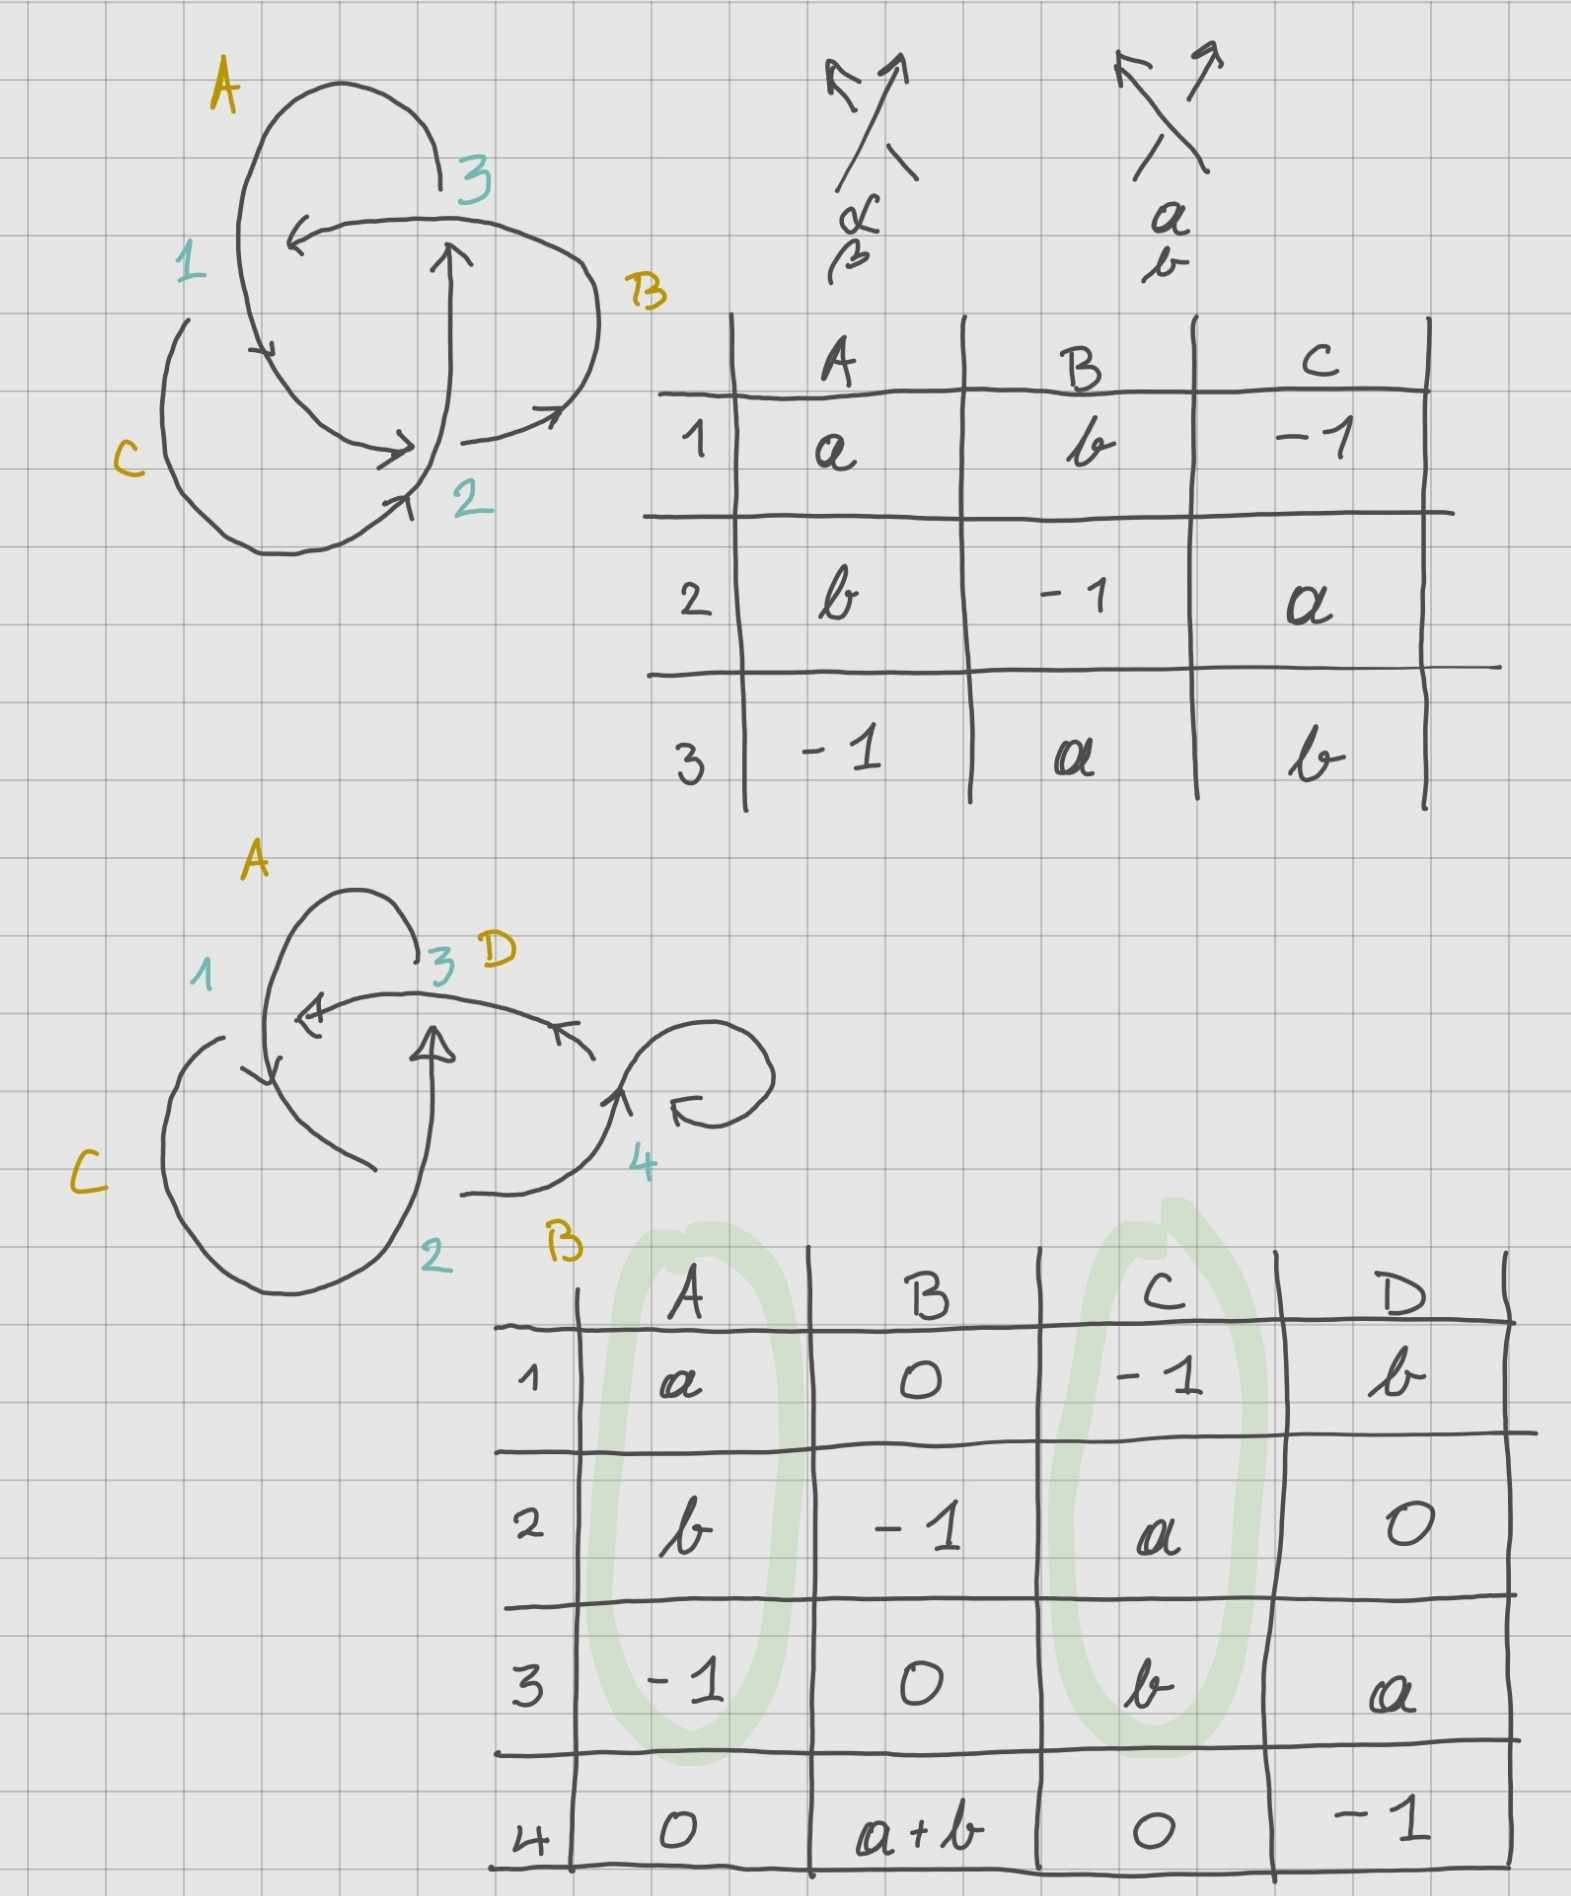
\includegraphics[width=\textwidth]{./rozdzialy/relacja_trefl_1.jpg}
\end{center}
\newpage 

Diagramiki skrzyżowań w prawym górnym rogu oznaczają, które skrzyżowanie ma $au+bi=-o$, a które $\alpha u+\beta i=-o$.

Niech $D$ będzie diagramem po usunięciu kinku, a $D'$ przed (góra-dół na rysunku). Dla prostoty $D:M^s\to N^x$ i $D:M^{s+1}\to N^{x+1}$ to macierze powstałe z odpowiednich diagramów.

Wtedy kolumny łuczków w $D$, które nie plączemy (ich jest $s-1$ sztuk) są bez zmiany, czyli 
$$D(M^{s-1})=D'(M^{s-1}).$$
Dodatkowo, jeśli $M_s$ jest łuczkiem, który zaplątaliśmy (ostatnia współrzędna, na obrazku troszkę nie wyszło), a $M_{s+1}$ łuczkiem, który przez zaplątanie powstał, to chcemy, żeby 
$$(D'(M_s)+ D'(M_{s+1}))\cap N^x=D(M_s),$$
gdzie to przecięcie po lewej stronie rozumiemy jako ograniczenie się do pierwszych $x$ współrzędnych powstałego wektora ($x+1$-sza to nowe skrzyżowanie).

\newpage 

\begin{center}
  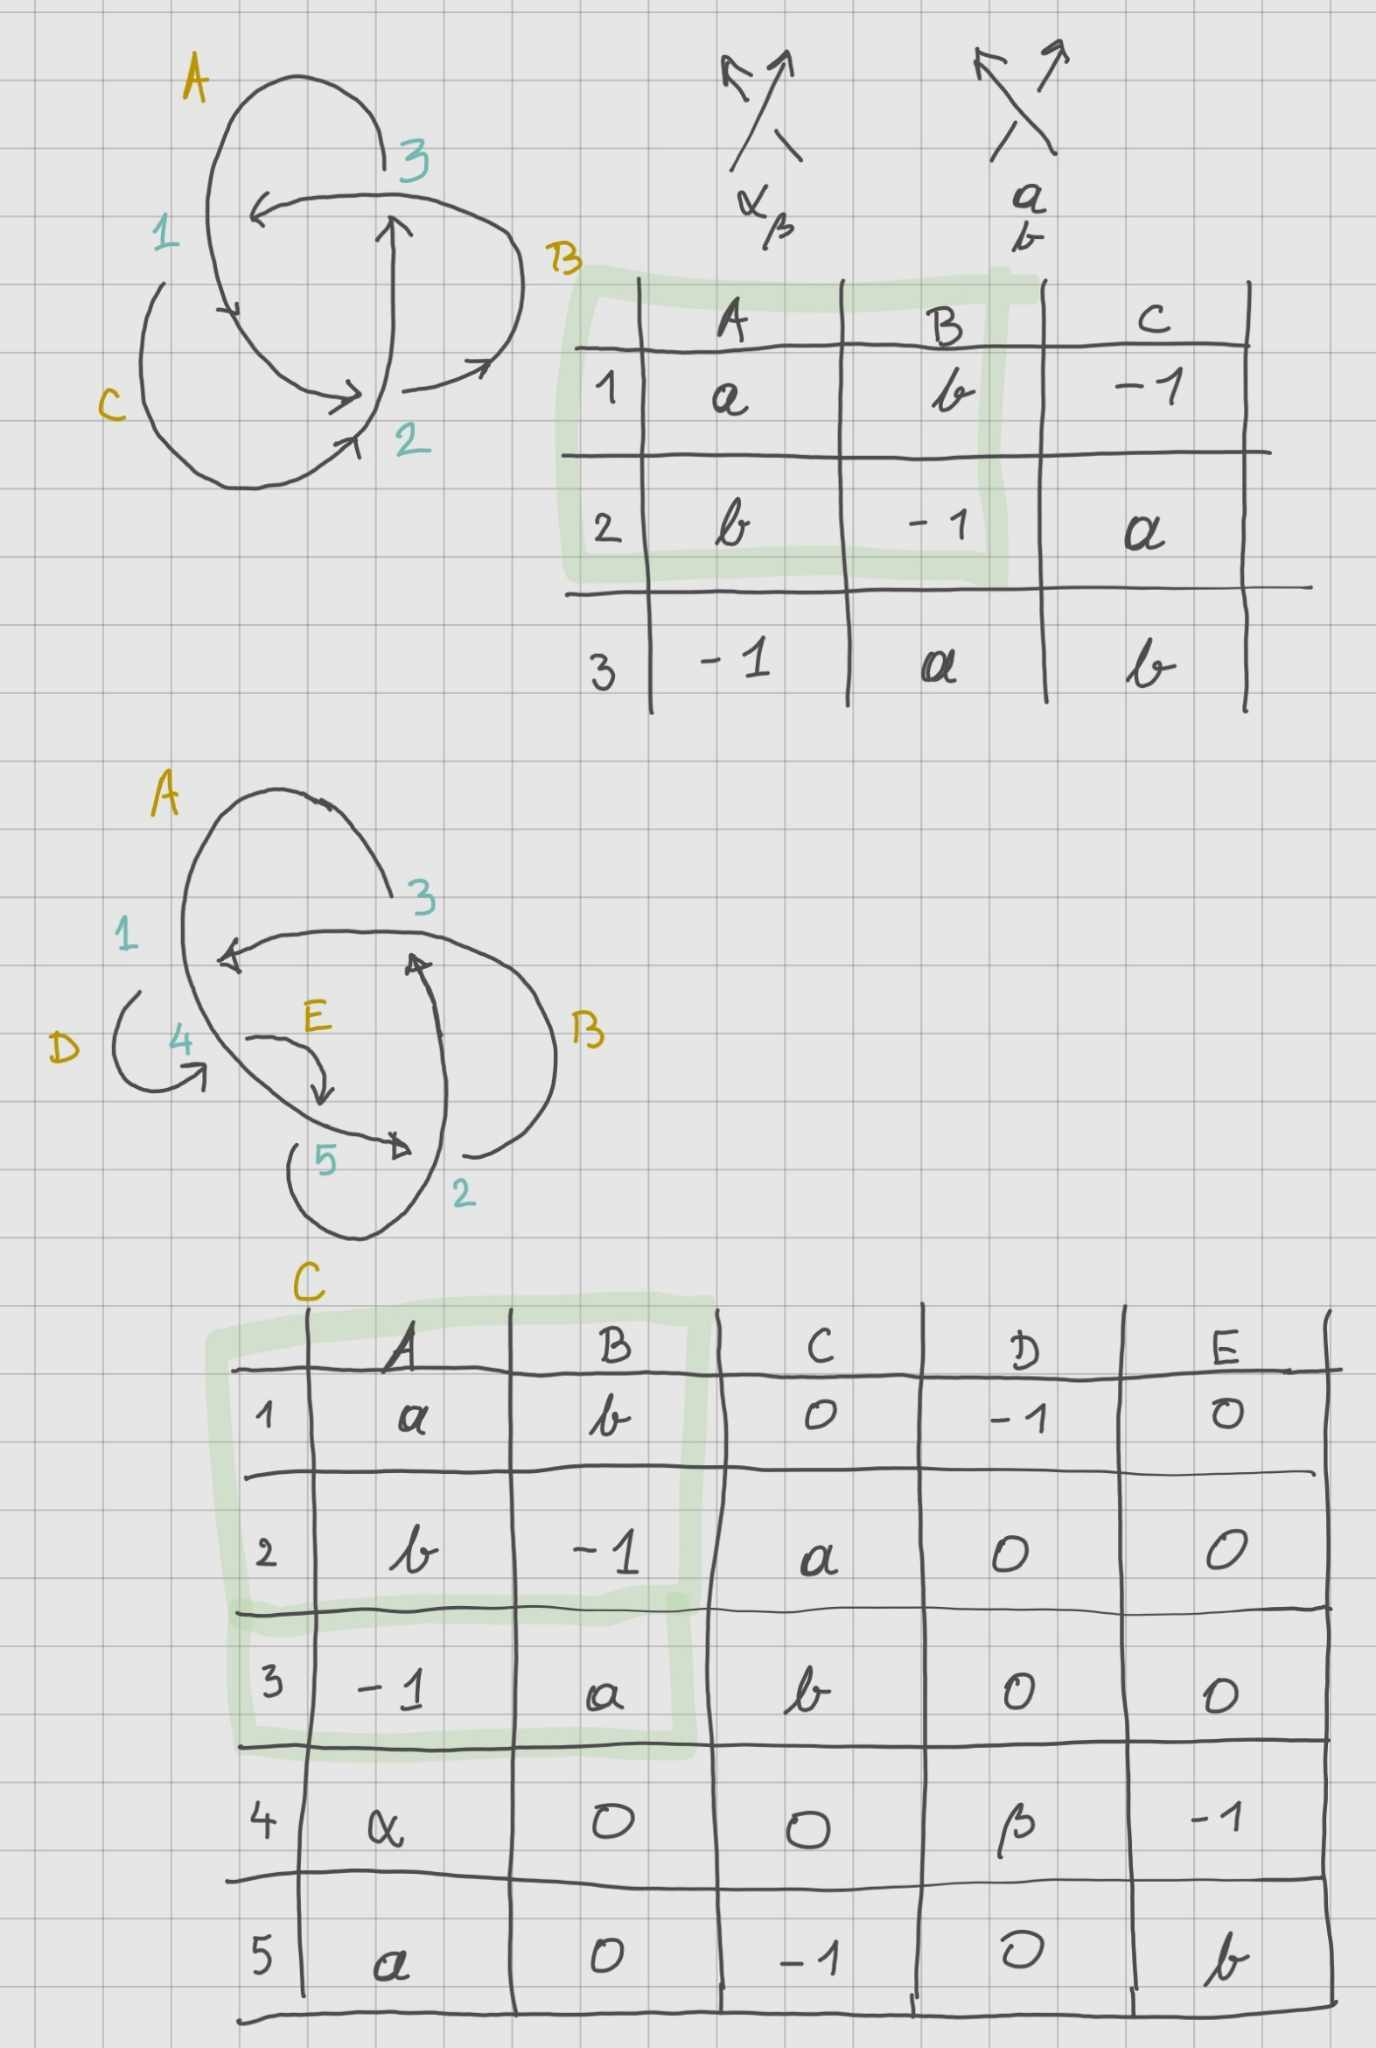
\includegraphics[width=\textwidth]{./rozdzialy/relacja_trefl_2.jpg}
\end{center}
\newpage 

W tym ruchu wyjęcia nitki spod spodu naruszyliśmy tylko jeden łuczek w diagramie po wyjęciu $D$ (diagram przed wyciągnięciem to $D'$). W takim razie, podobnie jak wcześniej chcemy
$$D(M^{s-1})=D'(M^{s-1})\cap N^x.$$
Możemy posunąć się dalej, i jeśli pierwsza nitka $M_1$ to ta, spod której wyjmowaliśmy, to chcemy 
$$(D(M^{s-1}), 0, 0)=D'(M^{s-1})-\omega_+(M_1, 0, 0)-\omega_-(M_1, 0, 0),$$
gdzie $\omega_\pm(u, i, o)$ to funkcja kolorująca odpowiadająca za każdy z rodzai skrzyżowań, jaki powstał przez wsunięcie pod $M_1$ nitki $M_s$. Oczywiście, musimy wiedzieć, które skrzyżowanie w $D'$ to który rodzaj skrzyżowania i umieścić $\omega_\pm(M_1,0,0)$ na odpowiedniej współrzędnej. 

Ta część wydaje mi się nieco brzydka. Po prostu chciałam jakoś zaakcentować fakt, że na ostatnich dwóch wierszach jedna nitka ma zawsze być górą i ma być górą na dwa różne sposoby.

Pozostaje powiedzieć, że fragmenty wsuniętej nitki dodają się do tego, co widzimy w nitce przed byciem wsuwaną:
$$D(M_s)=[D'(M_s)+D'(M_{s+1})+D'(M_{s+2})]\cap N^x$$

Pozostaje ostatni ruch Reidenmeistera oraz (chyba) napisanie tego samego dla odwrotnej orientacji.

\begin{center}
  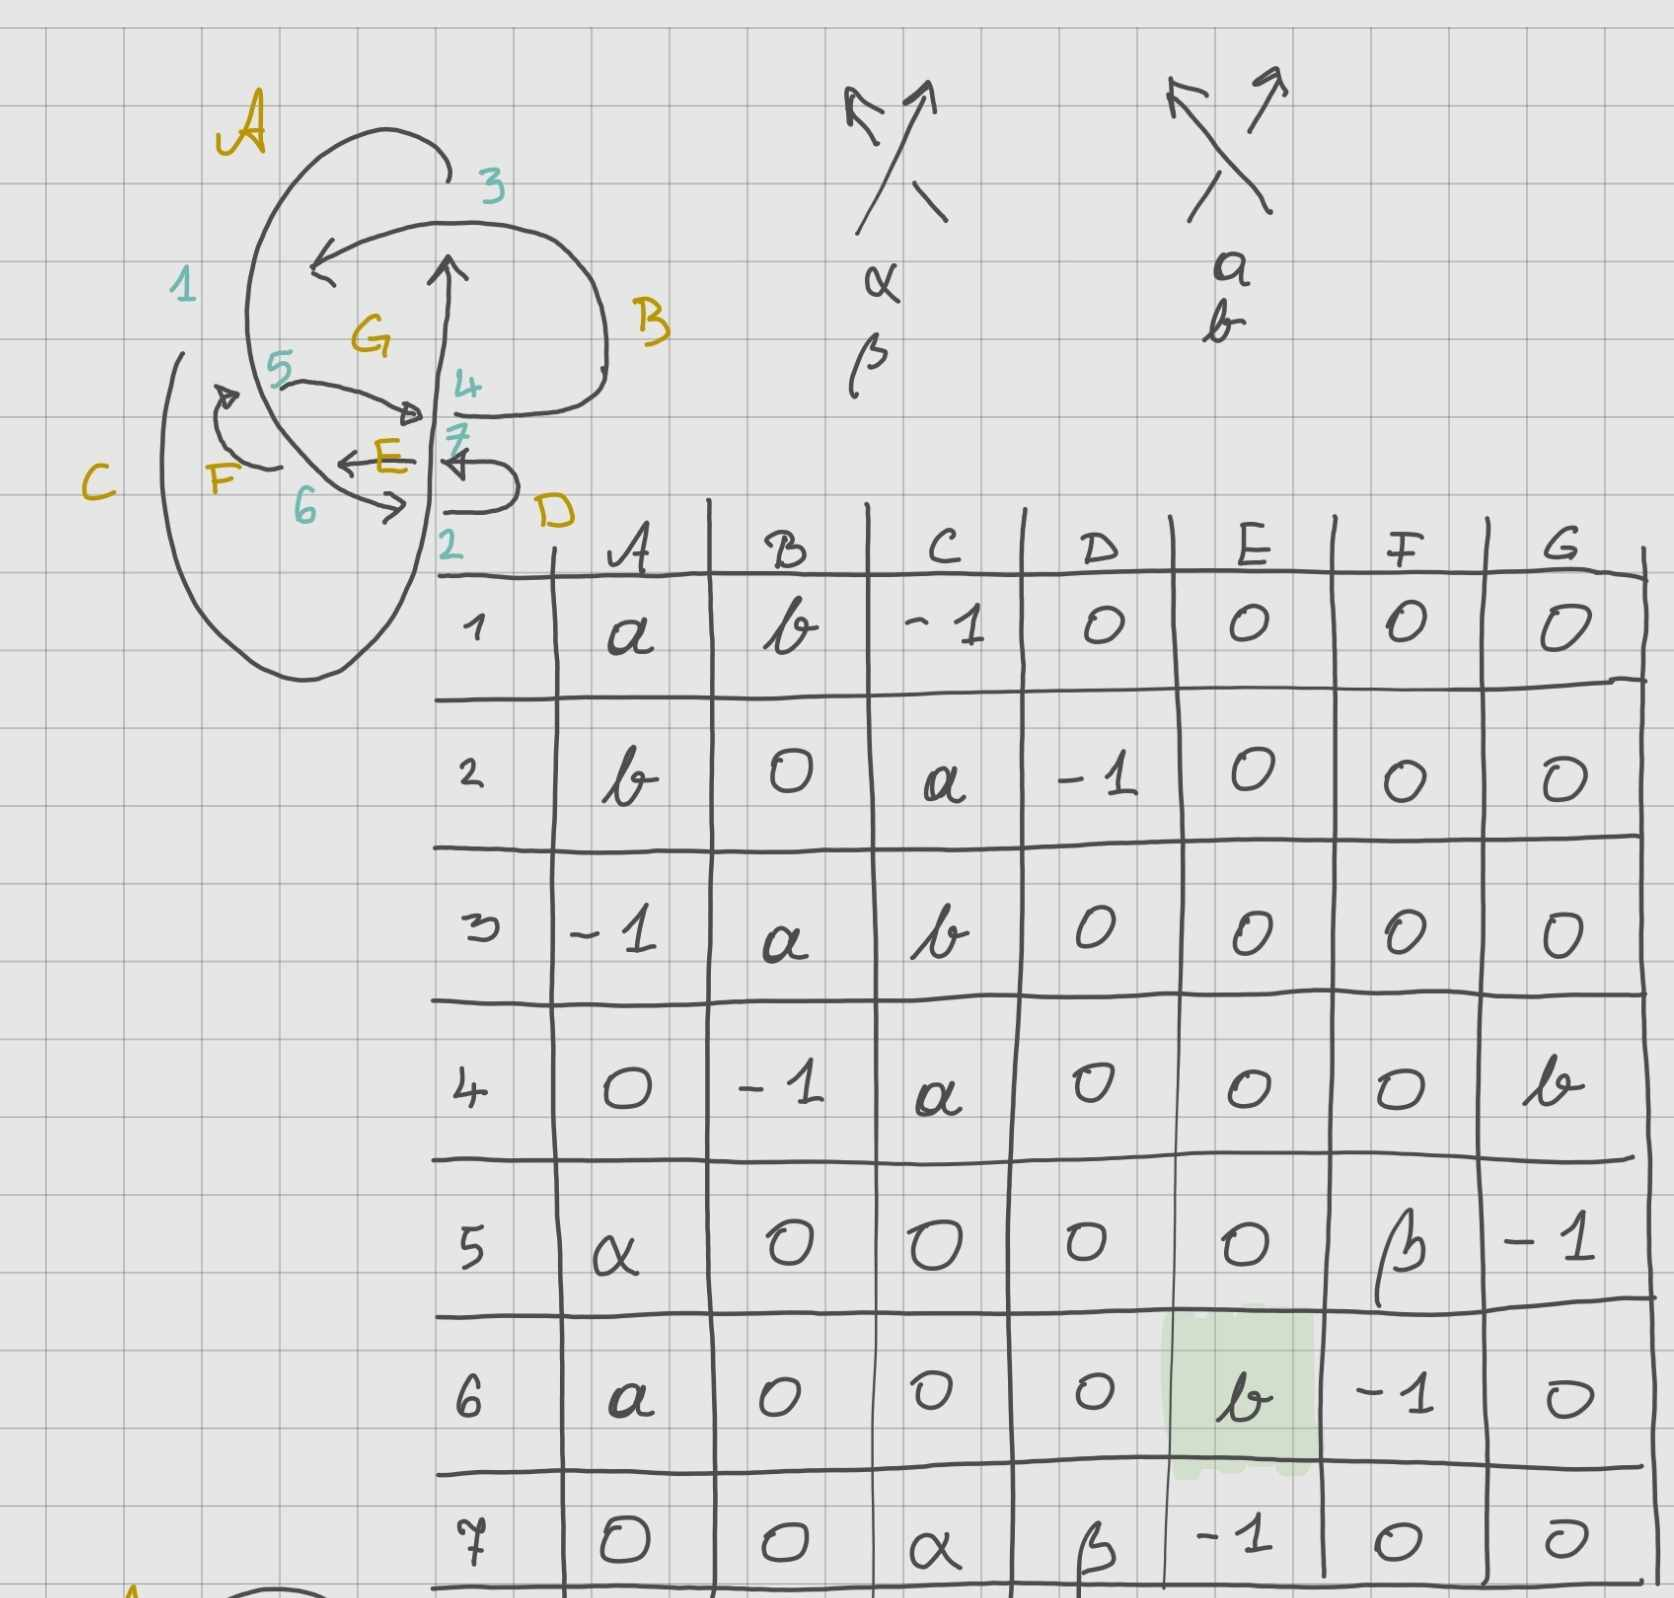
\includegraphics[width=\textwidth]{./rozdzialy/relacja_trefl_3.jpg}

  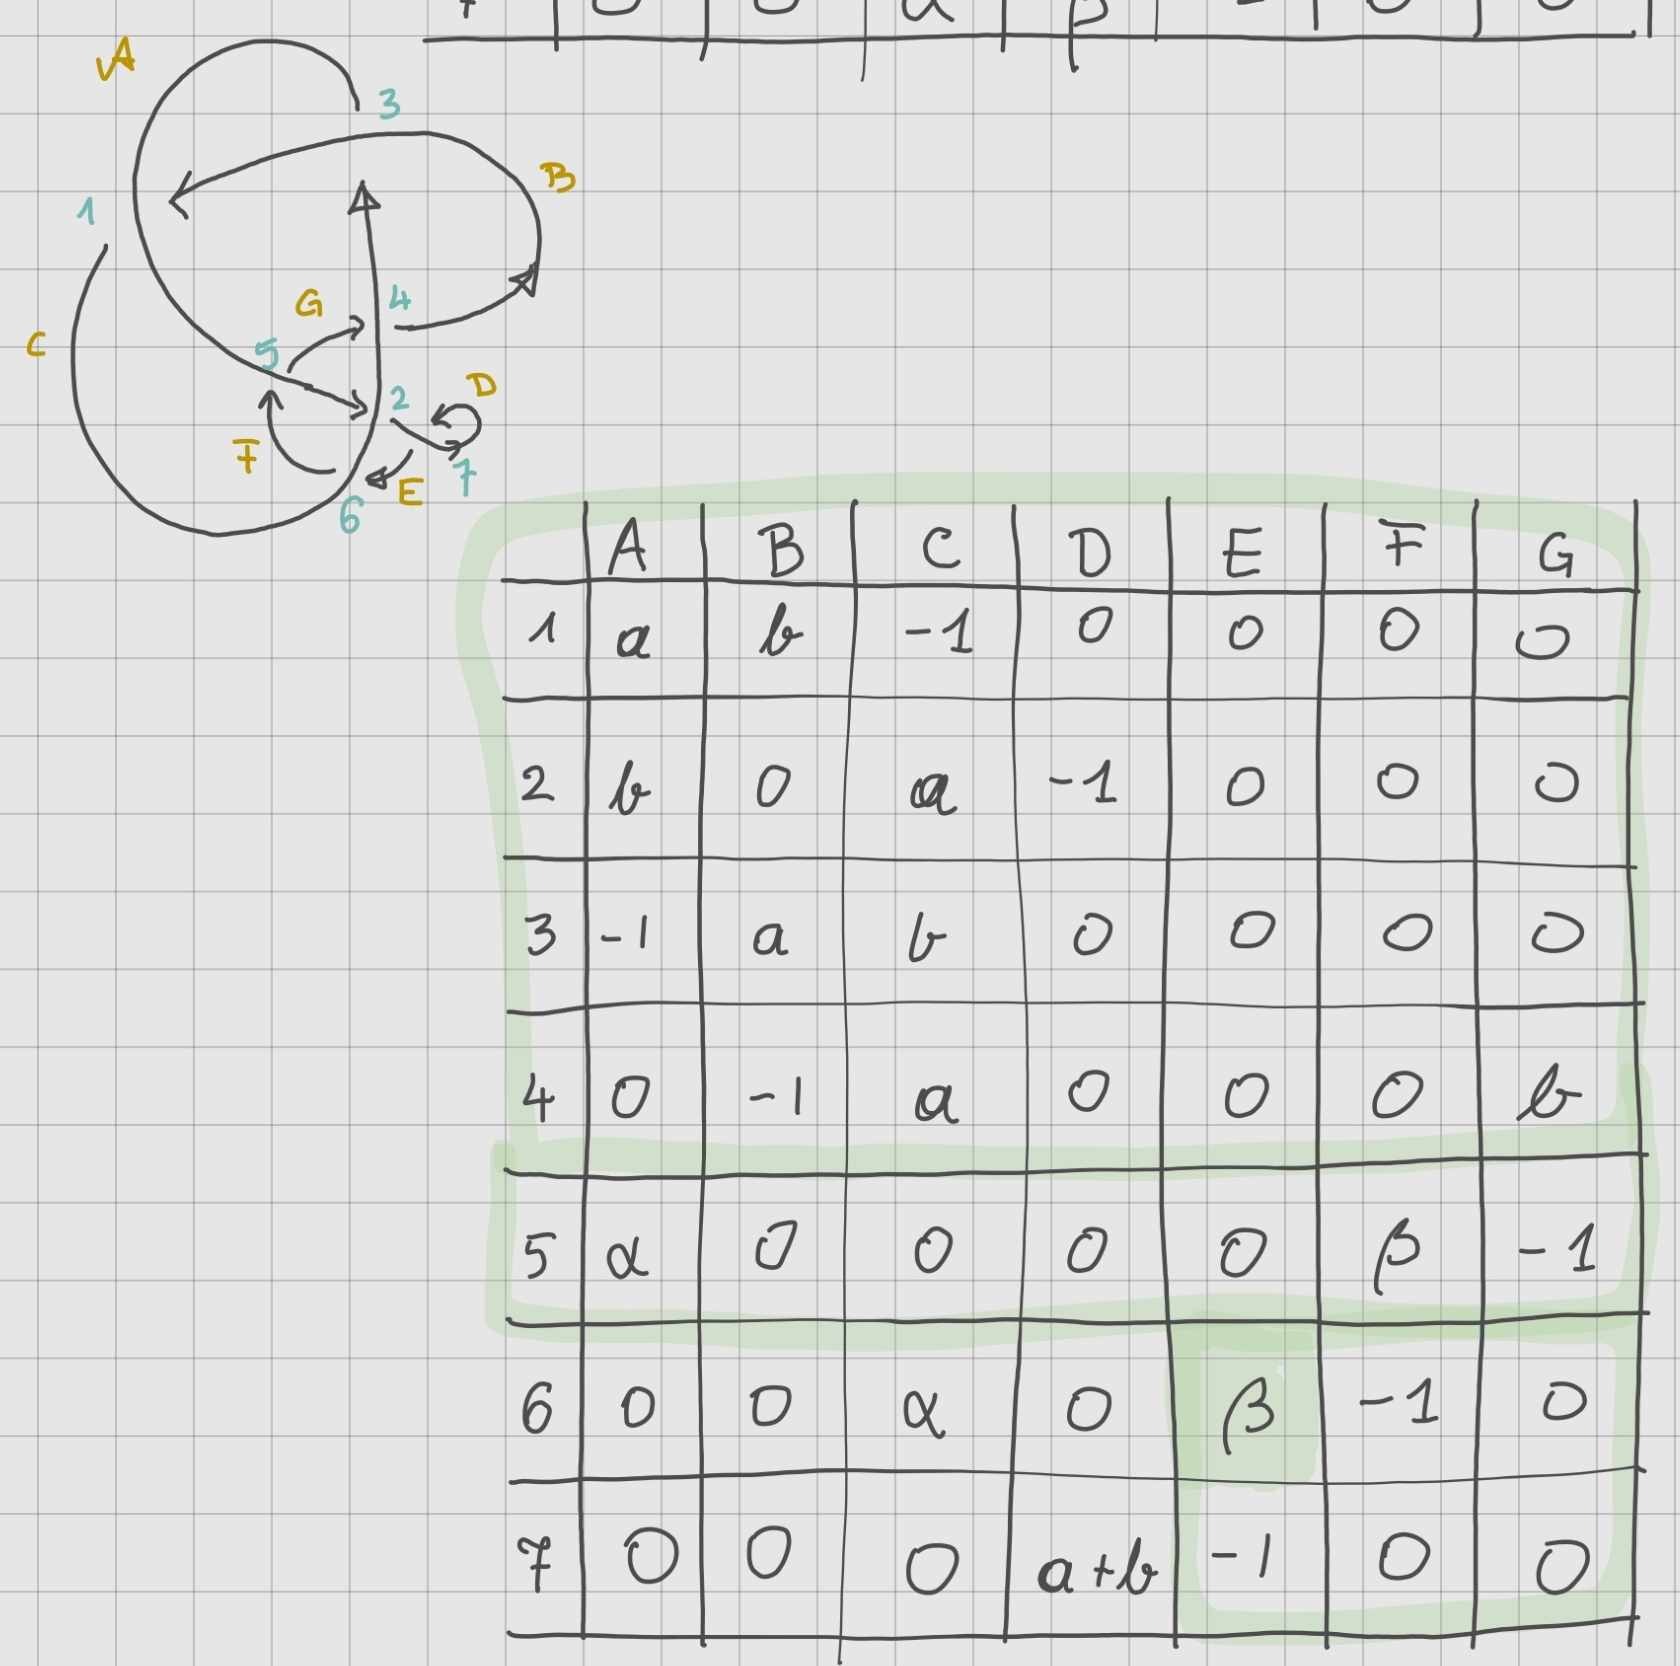
\includegraphics[width=\textwidth] {./rozdzialy/relacja_trefl_4.jpg}
\end{center}

\section{Troszkę grafu Gaussa}

\begin{center}
  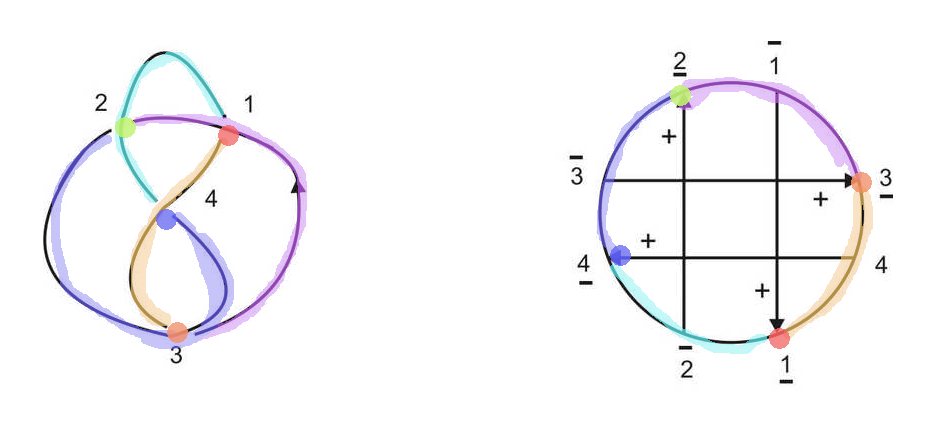
\includegraphics[width=\textwidth]{./rozdzialy/gauss_test.png}
\end{center}

Łuczki między grotami strzałek w grafie Gaussa odpowiadają łuczkom w grafie Reidemeistera.

To, gdzie idzie strzałka zaczynająca się gdzieś na łuczku mówi nam, nad którymi innymi dwoma łuczkami będzie on przechodził i w jakiej kolejności.

Nie wiem do końca jak będzie wtedy wyglądał kink.

To jedyna obserwacja jaką do tej pory miałam.
